\documentclass[a4paper, 11pt]{report}

\usepackage{a4wide,cite}
\usepackage[utf8]{inputenc}
\usepackage{amsmath, amsthm, amssymb, units, dsfont, algorithmicx, algpseudocode, nomencl}   % dsfont pro indikátor jevu
\usepackage[pdftex,
						pdfauthor={Jakub Klemsa},
						pdftitle={Models of self-assembling DNA nanostructures, Jakub Klemsa},
						pdfsubject={},
						pdfkeywords={Wang tiles, aTAM, Turing universality},
						pdfproducer={Jakub Klemsa},
						pdfcreator=dvipdf]{hyperref}
\usepackage{graphicx,color,tabularx,float}
\usepackage{fancyhdr}
\pagestyle{fancy}
\fancyhf{}
\fancyhead[L]{\slshape \rightmark} % \leftmark .. kapitola
\fancyhead[R]{\thepage}
\oddsidemargin=10mm   % jednostranný tisk !!!
\makenomenclature   % vyrobí nomenklaturu

\let\tmpitem\item
\renewcommand{\item}{\setlength{\itemsep}{2pt}\tmpitem}   % míň roztahovačný seznamy
\renewcommand{\labelitemi}{$\circ$}
%~ \def\refname{Li­teratura}   % záhadně nefunguje ???
%~ \frenchspacing   % údajně česká typografická pravidla

\theoremstyle{definition}
\newtheorem{example}{Example}[chapter]
%~ \newtheorem{definition}{Definice}[section]
%~ \newtheorem{predpoklad}{Předpoklad}[section]
%~ \newtheorem{tvrzeni}{Tvrzení}[section]
%~ \newtheorem{pozorovani}[tvrzeni]{Pozorování}
%~ \newtheorem{lemma}[tvrzeni]{Lemma}
%~ \newtheorem{dusledek}[tvrzeni]{Důsledek}
%~ \newtheorem{algoritmus}{Algoritmus}[chapter]

%~ \theoremstyle{remark} 
%~ \newtheorem{pozn}{Poznámka}[chapter]

\DeclareMathOperator*{\E}{E\,}   % operátor* bude umět používat \limit :)
\DeclareMathOperator{\de}{d\!}   % v integrálech
\renewcommand{\P}{\mathbb{P\,}}
\newcommand{\R}{\mathbb{R}}
\newcommand{\Z}{\mathbb{Z}}
\newcommand{\N}{\mathbb{N}}
\newcommand{\indicator}{\mathds{1}}
\newcommand{\powerset}[1]{\mathcal{P} ( #1 )}
\newcommand{\adob}[2]{#1 , \ldots , #2}

%%% VYHLEDAT A OPRAVIT !!! %%%%%%%%%%%%%%%%%%%%%%%%%%%%%%%%%%%%%%%%%%%%%
\let\haluz\relax
\let\hobza\relax
\haluz % program vlna nakonec!
% naučit se psát jednoduchý konsekventy! viz Adleman str. 3 nahoře: "Note that the labeling ..."
% taky opravit N-1 na N\!-\!1
% zkontrolovat \min \; ...
%%%%%%%%%%%%%%%%%%%%%%%%%%%%%%%%%%%%%%%%%%%%%%%%%%%%%%%%%%%%%%%%%%%%%%%%

%%% k vyplnění ZAČÁTEK -------------------------------------------------
\newcommand{\cvut}{ČESKÉ VYSOKÉ UČENÍ TECHNICKÉ V~PRAZE}
\newcommand{\fjfi}{Fakulta jaderná a fyzikálně inženýrská}
\newcommand{\km}{Katedra matematiky}
\newcommand{\obor}{Inženýrská informatika}
\newcommand{\minf}{Matematická informatika}
\newcommand{\TYPPRACE}{VÝZKUMNÝ ÚKOL}
\newcommand{\TypPrace}{Výzkumný úkol}
\newcommand{\mePrace}{mého výzkumného úkolu}
\newcommand{\rodPrace}{ho}

\newcommand{\nazevcz}{Modely sebeskládajících DNA nanostruktur}
\newcommand{\nazeven}{Models of self-assembling DNA nanostructures}
\newcommand{\autor}{Jakub Klemsa}
\newcommand{\vedouci}{Ing. Štěpán Starosta, Ph.D.}
\newcommand{\vedoucimu}{Ing. Štěpánu Starostovi, Ph.D.}
\newcommand{\pracovisteVed}{}
\newcommand{\konzultant}{---}
\newcommand{\rok}{2014}
\newcommand{\akadRok}{2013/2014}
\newcommand{\misto}{Praha}
\newcommand{\vMiste}{Praze}

\newcommand{\klicova}{Klíčová.}
\newcommand{\keyword}{Keywords.}
\newcommand{\abstrCZ}{Abstrakt CZ.}
\newcommand{\abstrEN}{Abstrakt EN.}
%%% k vyplnění KONEC ---------------------------------------------------


\begin{document}


\pagenumbering{roman}
\begin{titlepage}

%%% 1. úvodní strana
\thispagestyle{empty}
\begin{center}
	{\Large \cvut \\[12pt] \fjfi \\[260pt]}
	{\Huge \TYPPRACE}
\end{center}
\vfill
{
	\Large \misto, \rok \hfill \autor
}
\newpage


%%% 2. úvodní strana
\thispagestyle{empty}
\begin{center}
	{\Large \cvut \\[10pt] \fjfi \\[10pt] \km \\[40pt]}
	\includegraphics[height=75pt]{lev.pdf} \\[100pt]
	
	{\LARGE \TYPPRACE \\[60pt]}
	
	{\Large\bf \nazevcz \\[30pt]}
	
	{\Large\bf \nazeven}
\end{center}
\vfill
{
	\Large
	\begin{tabular}{ll}
	Vypracoval: & \autor\\[3pt]
	Školitel: & \vedouci\\[3pt]
	Akademický rok: & \akadRok
	\end{tabular}
}
\newpage


%%% sem přijde ofic. zadání
\thispagestyle{empty}
\Large
Na toto místo přijde svázat \textbf{zadání \mePrace}!

\vspace{4mm}
V~jednom z~výtisků musí být \textbf{originál} zadání, v~ostatních kopie.
\normalsize
\newpage


%%% prohlášení
\thispagestyle{empty}
~
\vfill
\noindent\textbf{Čestné prohlášení}
\vspace{0.5cm}

\noindent
Prohlašuji na tomto místě, že jsem předloženou práci vypracoval samostatně a že jsem uvedl veškerou použitou literaturu.
\vspace{1.5cm}

\noindent
\vspace{5mm}V \vMiste ~dne \today\hfill
	\begin{tabular}{c}
	. . . . . . . . . . . . . . . . . . . . . . .\\
	\autor
	\end{tabular}
\newpage


%%% poděkování
\thispagestyle{empty}
~
\vfill
\noindent\textbf{Poděkování}
\vspace{0.5cm}

\noindent
Děkuji \vedoucimu, za vedení \mePrace ~a za podnětné návrhy, které \rodPrace ~obohatily.

\begin{flushright}
\autor
\end{flushright}
\newpage


%%% abstrakt atp.
\thispagestyle{empty}

\begin{tabularx}{\textwidth}{lX}
  {\em Název práce:} & \bf \nazevcz \\[4mm]
  {\em Autor:} & \autor \\[4mm]
  {\em Obor:} & \obor \\[4mm]
  {\em Zaměření:} & \minf \\[4mm]
  {\em Druh práce:} & \TypPrace \\[4mm]
  {\em Vedoucí práce:} & \vedouci, \pracovisteVed \\[4mm]
  {\em Konzultant:} & \konzultant \\[4mm]
  {\em Abstrakt:} & \abstrCZ \\[4mm]
  {\em Klíčová slova:} & \klicova \\[20mm]

  {\em Title:} & \bf \nazeven \\[4mm]
  {\em Author:} & \autor \\[4mm]
  {\em Abstract:} & \abstrEN \\[4mm]
  {\em Key words:} & \keyword
\end{tabularx}
\newpage


%%% nomenklatura \haluz nefunguje
\thispagestyle{empty}
\printnomenclature
\newpage


%%% obsah
\tableofcontents
\thispagestyle{empty}

\end{titlepage}
\pagenumbering{arabic}


%%%%%%%%%%%%%%%%%%%%%%%%%%%%%%%%%%%%%%%%%%%%%%%%%%%%%%%%%%%%%%%%%%%%%%%%
%     Z A Č Á T E K   P R Á C E                                        %
%%%%%%%%%%%%%%%%%%%%%%%%%%%%%%%%%%%%%%%%%%%%%%%%%%%%%%%%%%%%%%%%%%%%%%%%


%%% ÚVODEM
\cleardoublepage\phantomsection   % cleardoublepage a phantomsection udělají že odkaz z obsahu vede NAD nadpis, jinak vede POD
\addcontentsline{toc}{chapter}{Prolog}
\chapter*{Prolog}

	1959: Feynman's visionary talk, \cite{feynman}; 
	
	The ground-breaking work was carried out by Adleman, \cite{adleman94}, who showed that DNA computation is practically feasible. In his experiment, Adleman used special DNA sequences for solving Hamiltonian Path Problem, one of the most typical NP-complete problems.
	
	... Extreme parallelism! But also possibility of errors.

\section*{Work overview}
	
	%%%%%%%%%%%%%%%%%%%%%%%%%%%%%%%%%%%%%%%%%%%%%%%%%%%%%%%%%%%%%%%%%%%%%%
	
	Chapter 1: Intro.\\
	Chapter 2: First of all I will describe models which exploit specific DNA structure.\\
	Chapter 3: Abstract Tile Assembly Model, temperature, 2D vs. 3D.\\
	Positive integers $\N$. \nomenclature{$\N$}{Positive integers.}
	
	% zkusíme Ramseyovo číslo R(5,5) ? :)
	% -> problém "Je R(n,n) větší než něco?" znamená pro odpověď ANO najít graf t.ž. neobsahuje K_n ani anti-K_n .. což je samo o sobě co-NP (neboli to je \exists \forall stroj .. \Sigma_2 jazyk, horní hranice pak je \Pi_2 jazyk)
	% 
	% NP vs co-NP .. co-NP přece nedává ne?

%%% KAPITOLA 1
\chapter{Introduction to DNA computation}
\label{chap:intro}

	
	1959: Feynman's visionary talk, \cite{feynman}; pros: extreme paralelism, cons: reliability.
	
	The ground-breaking work was carried out by Adleman, \cite{adleman94}, who showed that DNA computation is practically feasible. In his experiment, Adleman used special DNA sequences for solving Hamiltonian Path Problem, one of the most typical $\NP$-complete problems.
	
	... Extreme parallelism! But also possibility of errors.

\section*{Work overview}
	
	%%%%%%%%%%%%%%%%%%%%%%%%%%%%%%%%%%%%%%%%%%%%%%%%%%%%%%%%%%%%%%%%%%%%%%
	
	Chapter 1: Intro.\\
	Chapter 2: First of all we will describe models which exploit specific DNA structure.\\
	Chapter 3: Abstract Tile Assembly Model, temperature, 2D vs. 3D.\\
	Positive integers $\N$. \nomenclature{$\N$}{Positive integers.}
	
	% zkusíme Ramseyovo číslo R(5,5) ? :)
	% -> problém "Je R(n,n) větší než něco?" znamená pro odpověď ANO najít graf t.ž. neobsahuje K_n ani anti-K_n .. což je samo o sobě co-NP (neboli to je \exists \forall stroj .. \Sigma_2 jazyk, horní hranice pak je \Pi_2 jazyk)
	% 
	% NP vs co-NP .. co-NP přece nedává ne?

\section{Basic DNA principles}
	
	DNA (deoxyribonucleic acid) is a large biomolecule carrying living organisms' genetic information. Its most common structure is well known double-helix which consists of two strands connected by hydrogen bonds. These strands are biopolymers built up by {\em polymerase chain reaction} (PCR) from small units -- nucleotides. Each nucleotide consists of two parts: nitrogenous base and backbone molecules.
	\begin{description}
		\item[Nitrogenous bases] There are $4$ nucleobases in DNA ($+1$ in RNA): Adenine ({\bf A}), Thymine ({\bf T}), Cytosine ({\bf C}), Guanine ({\bf G}) and Uracil ({\bf U}) in RNA instead of Thymine in DNA. These molecules are responsible for making hydrogen bonds between strands in a manner following Watson-Crick complementarity: only {\bf A} -- {\bf T} and {\bf C} -- {\bf G} pairs can be formed.
		\item[Backbone molecules] Backbone of DNA strand is made of alternating deoxyriboses and phosphates. Phosphates only hold adjacent deoxyriboses, each deoxyribose moreover holds one nucleobase. Due to deoxyribose carbon numbering, DNA backbone has so called $5'$ and $3'$ ends, default reading order is $5'\rightarrow 3'$. DNA strands must be antiparallel so that nucleobases can connect.
	\end{description}

\section{Complexity, languages}
	
	\subsection{$O$ and other notations}
		
		Let us briefly remind $O$-, $o$-, $\Omega$-, $\omega$- and $\Theta$-notations for $f, g: \N \rightarrow \N$. We will denote $(\exists n_0 \in \N) (\forall n > n_0)$ shortly by $(\forall^* n)$ which can be read ``for almost all $n$''. Also $(\forall n_0 \in \N) (\exists n > n_0)$ will be denoted by $(\exists^\infty n)$ which can be read ``there exist infinitedly many $n$''.
		\begin{defn}
		\begin{align*}
			g \in O(f) &\iff (\exists C > 0) (\forall^* n) \bigl(g(n) < C f(n)\bigr) \\[5pt]
			g \in \omega^{(1)}(f) &\iff (\forall C > 0) (\exists^\infty n) \bigl(g(n) > C f(n)\bigr) \\[5pt]
			g \in \omega^{(2)}(f) &\iff (\forall C > 0) (\forall^* n) \bigl(g(n) > C f(n)\bigr) \\[5pt]
			g \in \Omega^{(1)}(f) &\iff (\exists C > 0) (\exists^\infty n) \bigl(g(n) > C f(n)\bigr) \\[5pt]
			g \in \Omega^{(2)}(f) &\iff (\exists C > 0) (\forall^* n) \bigl(g(n) > C f(n)\bigr) \\[5pt]
			g \in o(f) &\iff (\forall C > 0) (\forall^* n) \bigl(g(n) < C f(n)\bigr) \\[5pt]
			g \in \Theta(f) &\iff (\exists C_1, C_2 > 0) (\forall^* n) \bigl(C_1 f(n) \leq g(n) \leq C_2 f(n)\bigr) \\[5pt]
			g \sim f &\iff \lim\limits_{n\to\infty} \frac{g(n)}{f(n)} = 1
		\end{align*}
		\end{defn}
		
		\begin{remark}
			Note that there are two different definitions for omegas. $\Omega^{(1)}$ is equivalent to the orgininal definition introduced by Hardy \cite{hardy1914} which states
			\begin{equation*}
				f \in \Omega(g) \iff \limsup\limits_{n\to\infty}\frac{f(n)}{g(n)} > 0 .
			\end{equation*}
			The other, $\Omega^{(2)}$, was introduced by Knuth from good reasons described in \cite{knuth76}. In similar manner there are two definitions for $\omega$.
			
			Note that there are also some relations: the condition for $\Omega^{(1)}$ is negation of the condition for $o$ so these sets are complementary for given function $f$, similarly for $\omega^{(1)}$ and $O$. For the second variant one can easily check that $f\in\Omega^{(2)}(g)\iff g\in O(f)$ and $f\in\omega^{(2)}(g)\iff g\in o(f)$. There is also an equivalent condition for $\Theta$:
			\begin{equation*}
				g \in \Theta(f) \iff g \in O(f) \,\wedge\, f \in O(g) \iff g \in O(f) \,\wedge\, g \in \Omega^{(2)}(f) .
			\end{equation*}
			
			The condition for $g \sim f$ can be easily seen to be equivalent to $|f-g| \in o(g)$. In chapter~\ref{chap:problems} we will be mostly interested in this relation because it specifies the function better than $\Theta$. For example, $2n \in \Theta(n)$ but $2n \not\sim n$.
		\end{remark}
	
	\subsection{Studied complexities}
		
		\begin{defn}
			All the following complexities are considered as functions of problem size $n$:
			\begin{description}
				\item[Biostep complexity] will refer to the number of laboratory steps required to handle the computation, denoted by $Bs(n)$.
				\item[Binding complexity] will refer to the number of bindings in given computation, denoted by $Bnd(n)$.
				\item[Tile complexity] will refer to the number of different DNA tiles, denoted by $Ti(n)$.
				\item[Glue complexity] will refer to the number of different sticky-end sequences (commonly referred to as {\em glues}), denoted by $Gl(n)$. Each sequence with its Watson-Crick complement is considered as one glue.
			\end{description}
		\end{defn}
		
		\begin{remark}
			Note some properties of proposed complexities.
			\begin{description}
				\item[Ad biostep complexity] Adleman \cite{adleman95biostep} describes formally in his {\em unrestricted model} few types of such lab procedures -- {\em Separate, Merge, Detect} and {\em Amplify}, Winfree \cite{winfree_phd} adds another -- {\em Append}. And both of them remind that one biostep takes tens of minutes. Thus the only practically feasible DNA algorithms are those with $O(1)$ biostep complexity.
				\item[Ad binding complexity] Too high binding complexity leads to lower probability of correct computation $P_c$ because it holds $P_c(n) = (1-p_e)^{Bnd(n)} \approx\footnote{If reasonable.} \; 1-p_e \cdot Bnd(n)$ where $p_e$ denotes probability of erroneous binding.
				\item[Ad tile complexity] The higher tile complexity the more demanding it is to prepare required tiles.
				\item[Ad glue complexity] Higher glue complexity will require longer DNA sequences in the sticky ends. % which leads to hogher probability of erroneous binding $p_e$. %!% něco citovat co zminuje závislost p_e na dýlce sekvence, to přece musí rost ...
			\end{description}
		\end{remark}
	
	\subsection{Languages}
		
		\begin{defn}
			Let $\Sigma$ be an nonempty and finite set of {\em characters} which will be referred to as {\em alphabet}. Define set of {\em words} over alphabet $\Sigma$ as $\Sigma^* = \bigcup_{n\in\N_0}\Sigma^n$ and set of nonempty words as $\Sigma^+ = \bigcup_{n\in\N}\Sigma^n$. Empty word will be denoted by $\varepsilon$. {\em Language} ${\cal L}$ over alphabet $\Sigma$ is then just a set of words: ${\cal L} \subseteq \Sigma^*$. {\em Complement} of language $\cal L$ will be denoted by ${\cal\overline L} = \Sigma^* \setminus {\cal L}$.
		\end{defn}
		
		Let us briefly remind Chomsky hierarchy of languages generated by generative grammars. Denote alphabet of non-terminals by $N$, alphabet of terminals by $\Sigma$ and initial symbol by $I$.
		\begin{description}
			\item[Recursively enumerable (type 0)] Generated by unrestricted grammar rules.
			\item[Context-sensitive (type 1)] Grammar rules are either all of the form $\alpha A \beta \rightarrow \alpha \eta \beta$ where $\alpha,\,\beta\in (N\cup\Sigma)^*$, $A\in N$ and $\eta\in (N\cup\Sigma)^+$. Note that $\eta$ cannot be empty. Or, if we assume these rules without those having $I$ on the right hand side, then there is allowed also the rule $I\rightarrow \varepsilon$.
			\item[Context-free (type 2)] All grammar rules are of the form $A\rightarrow\eta$ where $A\in N$ and $\eta\in (N\cup\Sigma)^*$. Note that $\eta$ can be empty.
			\item[Regular (type 3)] Grammar rules are either all of the forms $A\rightarrow bB$ and $A\rightarrow b$ where $A,\,B\in N$ and $b\in\Sigma$. Or, if we assume these rules without those having $I$ on the right hand side, then there is allowed also the rule $I\rightarrow \varepsilon$.
		\end{description}
		
		\begin{remark}
			Note that given an alphabet $\Sigma$ the set of all words $\Sigma^*$ is countable. Moreover, one can sort $\Sigma^*$ first by word length, then lexicographically thus it is easy to define desired bijection $f: \N \leftrightarrow \Sigma^* $.
			
			Formal language ${\cal L}$ can then be viewed as a boolean function $g: \N \rightarrow \{0,1\}$ defined as
			$g(n) = 1 \iff f(n)\in {\cal L}$.
		\end{remark}
		
		% přidat čim je co rozpoznávatelný?
		% abeceda \Sigma -> {0, 1} ??
	
	\subsection{$\P$, $\NP$ and other}
	\label{sec:PNP}
		
		This section describes few classes of languages from the resource-consumption point of view. There exist many equivalent definitions, these are taken from \cite{book_comp}. % The first set of definitions is very straightforward and thus can be used for propositions.
		
		\begin{defn}\label{def:P}
			${\cal L} \subseteq \Sigma^*$. ${\cal L} \in \P \iff \bigl(\exists p \in {\cal P}\bigr) \bigl(\exists \textnormal{ deterministic Turing machine } M\bigr)\\ \bigl(\forall x \in \Sigma^*\bigr) \bigl(x \in {\cal L} \iff M \textnormal{ accepts } x \textnormal{ in time } \leq p(|x|)\bigr)$.
		\end{defn}
		
		\begin{defn}\label{def:NP}
			${\cal L} \subseteq \Sigma^*$. ${\cal L} \in \NP \iff \bigl(\exists p, q \in {\cal P}\bigr) \bigl(\exists \textnormal{ deterministic Turing machine } M\bigr)\\ \bigl(\forall x \in \Sigma^*\bigr) \Bigl(x \in {\cal L} \iff \bigl(\exists y \in \Sigma^{p(|x|)}\bigr) \bigl(M \textnormal{ accepts } (x,y) \textnormal{ in time } \leq q(|x|+|y|)\bigr)\Bigr)$.\\
			Such $y$ will be referred to as {\em certificate} for $x$ (with respect to $\cal L$ and $M$).
		\end{defn}
		
		\begin{defn}\label{def:coNP}
			${\cal L} \subseteq \Sigma^*$. ${\cal L} \in \coNP \iff \bigl(\exists p, q \in {\cal P}\bigr) \bigl(\exists \textnormal{ deterministic Turing machine } M\bigr)\\ \bigl(\forall x \in \Sigma^*\bigr) \Bigl(x \in {\cal L} \iff \bigl(\forall y \in \Sigma^{p(|x|)}\bigr) \bigl(M \textnormal{ accepts } (x,y) \textnormal{ in time } \leq q(|x|+|y|)\bigr)\Bigr)$.
		\end{defn}
		
		The second possibility is to first define general classes $\DTime$, $\NTime$, $\DSpace$ and $\NSpace$ and after that to use their special case. Remind how Non-deterministic Turing machine (NTM) differs from Deterministic Turing machine (DTM):
		\begin{itemize}
			\item it is allowed to have ambiguous transition function,
			\item it has two types of terminal states: accepting $q_{accept}$ and halting without accepting $q_{halt}$ (not rejecting!). We say it accepts input $x$ iff there {\em exists} a sequence of decisions ending in $q_{accept}$, it declines $x$ iff {\em for every} sequence of decisions reaches $q_{halt}$.
		\end{itemize}
		
		%!% tady je problém s negací v D---- ptž polynom časově konstruovatelnej je ale co když f(n) neni že ... ale asi mi to neva ...
		\begin{defn}\label{def:DTime}
			$\DTime\bigl(f(n)\bigr) = \bigl\{ {\cal L}\textnormal{ language} \bigm| (\exists \textnormal{ deterministic Turing machine }M)\\ (\forall x\in\Sigma^*)\bigl(x\in{\cal L} \iff M\textnormal{ accepts }x\textnormal{ in time }\leq f(|x|)\bigr) \bigr\}$.\\
			Other classes are defined in a very similar manner: time $\leftrightarrow$ space, deterministic $\leftrightarrow$ non-deterministic.
		\end{defn}
		
		\begin{defn}
			$\P = \bigcup\limits_{k\in\N} \DTime(n^k)$ and $\NP = \bigcup\limits_{k\in\N} \NTime(n^k)$.
		\end{defn}
		
		\begin{defn}
			$ {\cal L} \in \coNP \iff {\cal\overline L} \in \NP $.
		\end{defn}
		
		\begin{note}
			$\NP\subseteq\powerset{\Sigma^*}$ so the notation $\coNP$ might be confusing. Note that $\coNP$ is {\em not} a complement to $\NP$ as a set of languages.
		\end{note}
		
		\begin{remark}
			In case of $\P$ there is no ``co'' version. It follows from ${\cal L} \in \P \iff \overline{\cal L} \in \P$. This can be easily seen because deterministic Turing machine is capable of negation with the same time resources, non-deterministic is not known to. Note that Immerman--Szelepcsényi theorem states possibility of non-deterministic Turing machine negation in limited {\em space}: ${\cal L} \in \NSpace(s(n)) \iff \overline{\cal L} \in \NSpace(s(n))$ for $s(n) \geq \log(n)$.   %!% problematickej: \footnote{Since $\P = \NP = \coNP$ is not known.}
		\end{remark}
		
		\begin{thm}
			All the previous definitions of $\P$, $\NP$ and $\coNP$ are equivalent.
		\end{thm}
		
		\begin{defn}
			We say that language ${\cal L}_1$ is {\em polynomial-time Karp reducible} to ${\cal L}_2$ and denote ${\cal L}_1\propto{\cal L}_2 \iff \exists$ polynomial-time computable function $f:\Sigma^*\rightarrow\Sigma^*$ such that $(\forall x\in\Sigma^*)(x\in{\cal L}_1\iff x\in{\cal L}_2)$.
		\end{defn}
		
		\begin{defn}
			${\cal L}\in\NPH \iff (\forall{\cal L'}\in\NP)({\cal L'}\propto{\cal L})$.
		\end{defn}
		
		\begin{defn}
			${\cal L}\in\NPC\iff{\cal L}\in\NP\cap\NPH$.
		\end{defn}
		
		\begin{note}
			If we found a polynomial-time algorithm for {\em any} $\NPC$ language, it would hold $\P=\NP$ which is not believed to be true. Thus supposed that $\P\neq\NP$ there does not exist a polynomial algorithm for any $\NPC$ language.
		\end{note}
		
		\begin{example}\label{exm:npc}
			Remind some popular $\NPC$ problems: boolean formula satisfability ($\mathsf{SAT}$), Hamiltonian path problem ($\mathsf{HPP}$), graph $3$-coloring, graph $k$-independent set, graph $k$-clique, graph $k$-vertex cover, subset sum and many others.
			
			On the other hand there are few interesting problems which are not known to belong either to $\P$ nor to $\NPC$, one of them is graph isomorphism problem.
		\end{example}
		
		% poly-time hierarchy ... book pg. 93
		
		To define probabilistic classes of languages ($\BPP$, $\RP$, $\coRP$ and $\ZPP$) we will remind the concept of Probabilistic Turing machine (PTM). Like NTM it is allowed to have ambiguous transition function, moreover, in every state there is defined a transition probability and it can have another terminal state $q_{reject}$.
		
		We say that PTM $M$
		\begin{itemize}
			\item decides language $\cal L$ iff for every $x\in\Sigma^*$ the probability of halting in correct state (i.e. $q_{accept}$ for $x\in{\cal L}$ and $q_{reject}$ for $x\notin{\cal L}$) is higher than $\nicefrac{2}{3}$.
			\item decides language $\cal L$ in time $t(n)$ iff $M$ decides language $\cal L$ and for every $x\in\Sigma^*$ it halts in time $\leq t(|x|)$.
		\end{itemize}
		Now we can define those classes, note that it would be possible to use again two types of definition like above.
		
		% příp. pg 121 .. tam je alternativní def
		
		\begin{defn}\label{def:BPTime}
			$\BPTime\bigl(f(n)\bigr) = \bigl\{ {\cal L}\textnormal{ language} \bigm| (\exists \textnormal{ probabilistic Turing machine }M)\\ \bigl(M\textnormal{ decides }{\cal L}\textnormal{ in time }\leq f(|x|)\bigr) \bigr\}$.
		\end{defn}
		
		\begin{defn}
			$\BPP = \bigcup\limits_{k\in\N} \BPTime(n^k)$.
		\end{defn}
		
		\begin{defn}
			$\RTime\bigl(f(n)\bigr) = \bigl\{ {\cal L}\textnormal{ language} \bigm| (\exists \textnormal{ probabilistic Turing machine }M)\\ (\forall x\in\Sigma^*)\bigl(M \textnormal{ halts in time } \leq f(|x|) \;\wedge\; x\in{\cal L} \then \prob(M\textnormal{ accepts }x) \geq \nicefrac{2}{3} \;\wedge\\ x\notin{\cal L} \then \prob(M\textnormal{ accepts }x) = 0 \bigr) \bigr\}$.
		\end{defn}
		
		\begin{defn}
			$\RP = \bigcup\limits_{k\in\N} \RTime(n^k)$.
		\end{defn}
		
		\begin{defn}
			$ {\cal L} \in \coRP \iff {\cal\overline L} \in \RP $.
		\end{defn}
		
		\begin{remark}
			$\BPP$ allows PTM to make both wrong decisions (for $x\in\cal L$ as well as for $x\notin\cal L$), on the other hand $\RP$ does not allow error for $x\notin\cal L$ and $\coRP$ does not allow error for $x\in\cal L$. Following class $\ZPP$ (from {\em zero error}) does not allow any error, it only allows halting neither with accepting nor with rejecting.
		\end{remark}
		
		%!% proč mam pocit že to maj v book blbě definovaný? takle by to znamenalo P=ZPP. líp u majerecha!
		
		\begin{defn}
			$\ZPTime\bigl(f(n)\bigr) = \Bigl\{ {\cal L}\textnormal{ language} \Bigm| \bigl(\exists \textnormal{ probabilistic Turing machine }M\bigr)\\ \bigl(\forall x\in\Sigma^*\bigr)\Bigl(M \textnormal{ halts in time } \leq f(|x|) \;\wedge\\ \bigl(x\in{\cal L} \then \prob(M\textnormal{ accepts }x) \geq \nicefrac{2}{3} \,\wedge\, \prob(M\textnormal{ rejects }x) = 0 \bigr) \;\wedge\\ \bigl(x\notin{\cal L} \then \prob(M\textnormal{ rejects }x) \geq \nicefrac{2}{3} \,\wedge\, \prob(M\textnormal{ accepts }x) = 0 \bigl) \Bigr) \Bigr\}$.
		\end{defn}
		
		\begin{defn}
			$\ZPP = \bigcup\limits_{k\in\N} \ZPTime(n^k)$.
		\end{defn}
		
		\begin{thm}
			\begin{equation*}
				{\cal L}_{1,2}\in\ZPP\then{\cal\overline L}_1,\,{\cal L}_1\cap{\cal L}_2,\,{\cal L}_1\cup{\cal L}_2\in\ZPP .
			\end{equation*}
		\end{thm}
		
		\begin{thm}
			\begin{align*}
				\P \subseteq \ZPP &= \RP \cap \coRP , \\
				\RP &\subseteq \NP\cap\BPP , \\
				\coRP &\subseteq \coNP\cap\BPP .
			\end{align*}
		\end{thm}
		
		% PP, \#P, PSpace ..? Maybe also polynomial hierarchy: $\Sigma_k P$ and $\Pi_k P$ languages (alternating Turing machine with bounded alternation, \cite{kozen06}). Might be nice to show what DNA computation is capable of.
		
		% SAT: Lipton's contribution using $m$ biosteps ($m = \#clauses$), \cite{lipton95}, Lipton's set of speedup problems, \cite{lipton96speedup}.
		% Energy efficiency (Adleman).

% úvod o kapitole, přehled

\section{Strand models}
	
	There exist (can be synthesized) many types of molecules, well described in Winfree \cite{winfree_phd} even with their inception reaction. The most important structures are linear strands (sections \ref{sec:lin_strands}, \ref{sec:adleman}, figure \ref{fig:linear}), dendrimer structures (section \ref{sec:dendrimer}, figure \ref{fig:dendrimer}) and double crossover molecules (section \ref{sec:double_crossover}, figure \ref{fig:double_crossover}).
	\begin{note}\label{note:untwist}
		DNA naturally forms double-helices which would be confusing in figures so there will mostly appear schemes of ``untwisted'' molecules, double crossover molecules will be described more precisely. % nebo snad unscrewed?
	\end{note}
	
	
	%~ \subsection{Single-stranded molecules}
		%~ 
		%~ As we noted before, the only feasible methods are those computing in $O(1)$ biosteps.
		%~ 
		%~ SAT in $O(1)$ biosteps etc.
	
	%~ \subsection{Double-stranded molecules}
	
	\subsection{Linear strands}
	\label{sec:lin_strands}
		
		\begin{figure}[H]
		\begin{center}
			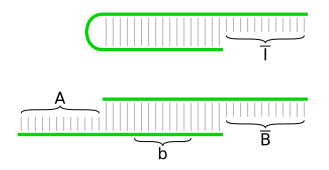
\includegraphics[width=0.502\textwidth]{./figures/strand_types/linear.pdf} % {šířka v mm}/370 je to původně
			\caption{Linear strands: Strand for initial symbol $I$ and strand for rule $A\rightarrow bB$.}
			\label{fig:linear}
		\end{center}
		\end{figure}
		
		Equivalent to regular languages: Winfree pg 53.
	
	\subsection{Adleman's experiment}
	\label{sec:adleman}
		
		Adleman showed in his ground-breaking work \cite{adleman94} that DNA molecules are really capable of computation. He exploited that huge parallelism possible in DNA computation for one of the most fundamental $\NP$-complete problems -- the Hamiltonian Path Problem (HPP) in directed graph with designated vertices $v_{begin}$ and $v_{end}$.
		
		Let us remind this type of HPP. Given a directed graph $G_n$ with $n$ vertices and two designated vertices $v_{begin}$ and $v_{end}$, the problem is to answer whether there exists an oriented path from $v_{begin}$ to $v_{end}$ through the graph such that the path visits every vertex. Note that {\em path} cannot visit any vertex more than once from definition.
		
		\begin{figure}[H]
		\begin{center}
			\includegraphics{./figures/adleman_graph.pdf}
			\caption{Adleman's original graph.}
			\label{fig:adleman_graph}
		\end{center}
		\end{figure}
		
		Adleman originally used a graph with seven vertices shown in figure \ref{fig:adleman_graph}. It can be seen that the path $0 \rightarrow 1 \rightarrow 2 \rightarrow 3 \rightarrow 4 \rightarrow 5 \rightarrow 6$ is Hamiltonian\footnote{Note that it can be re-labelled such a nice way without loss of generality.}.
		
		Adleman first presents this non-deterministic five-step algorithm, whose steps are then described in terms of DNA manipulations:
		\begin{description}
			\item[Step 1] Generate random paths through the graph.
			\item[Step 2] Keep only those paths that begin with $v_{begin}$ and end with $v_{end}$.
			\item[Step 3] If the graph has $n$ vertices, then keep only those paths that enter exactly $n$ vertices.
			\item[Step 4] Keep only those paths that enter all of the vertices of the graph at least once.
			\item[Step 5] If any paths remain, say ``Yes''; otherwise, say ``No.''\footnote{This is the original version, I would rectify the fifth step: If any paths remain, say ``Yes''; otherwise say ``{\em I do not know}''. That is because it may happen that there exists a valid path but unfortunately it did not assemble or got lost. Note the similarity to $\NP$ versus $\coNP$, see section \ref{sec:PNP}.} %!% citaci, někdo to už taky kritizoval
		\end{description}
		To see % sloveso od insight ?
		how DNA can compute, let us describe this example more precisely. The computation itself (meaning the inception of the final solution) is hidden in Step 1. Each vertex $i$ is associated with a random\footnote{We will expect those sequences to be different enough.} $20$-mer sequence of DNA, let us denote its $5'\rightarrow 3'$ orientation by $O_i$, its 10-mer prefix by $p_i$ and its 10-mer suffix by $q_i$. Each edge $i\rightarrow j$ is then associated with $\overline{q_i p_j}$ sequence with reverse backbone orientation ($3'\rightarrow 5'$) where $\overline{q_i}$ stands for Watson-Crick complementary word. There is an exception for $i=begin$ and $j=end$: instead of $\overline{q_{begin} p_j}$ there is $\overline{O_{begin} p_j}$ and in a similar way for $j=end$.
		
		\begin{figure}[H]
		\begin{center}
			\includegraphics{./figures/adleman_strands.pdf}
			\caption{Example of assigned sequences.}
			\label{fig:adleman_strands}
		\end{center}
		\end{figure}
		
		It can be easily seen that all correctly bonded double-strands correspond with a valid walk through $G_n$. Moreover, all complete double-strands represent a valid walk from $v_{begin}$ to $v_{end}$ through $G_n$.
		
		All the other steps are fully described in \cite{adleman94}. The most important thing is that the most time-demanding step is Step 4. In this step one has to purify the product of Step 3 with a {\em biotin-avidin magnetic beads system}. This process extracts consequently for every vertex $i$ only those DNA strands which contain a substring representing vertex $i$. Thus this algorithm has biostep complexity $O(n)$ which we considered unfeasible. Better solution with biostep complexity $O(1)$ was introduced by Winfree \cite{winfree_phd}, see section \ref{sec:double_crossover}.
	
	\subsection{Dendrimer structures}
	\label{sec:dendrimer}
		
		\begin{figure}[H]
		\begin{center}
			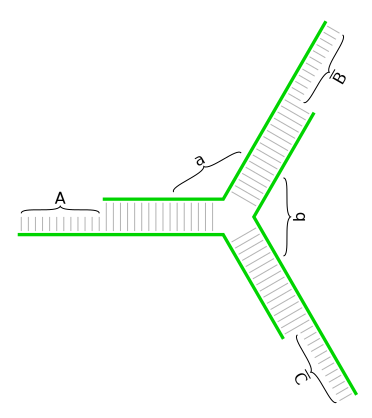
\includegraphics[width=0.568\textwidth]{./figures/strand_types/dendrimer.pdf}
			\caption{Dendrimer structure for rule $A\rightarrow aBbC$.}
			\label{fig:dendrimer}
		\end{center}
		\end{figure}
		
		Equivalent to context-free languages: Winfree pg 54.
	
	\subsection{Double crossover molecules}
	\label{sec:double_crossover}
		
		Double crossover molecules are the most important ones. Though they are more complicated they are still very rigid \cite{seeman93}. Moreover they are theoretically capable of universal computation because they can form 2D tilings\footnote{See figure \ref{fig:DNA_assembly} and note how this type of molecules form tilings.} and thus they can simulate blocked cellular automaton \cite{winfree_phd}. As we mentioned in note \ref{note:untwist} we will also describe their inner structure. % universal computation: Winfree pg 57
		
		\begin{figure}[H]
		\begin{center}
			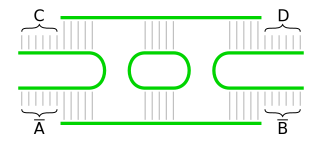
\includegraphics[width=0.492\textwidth]{./figures/strand_types/double_crossover.pdf}
			\caption{Double crossover molecule scheme.}
			\label{fig:double_crossover}
		\end{center}
		\end{figure}
		
		There are many possibilities how those strands can be twisted and connected. The most common ones are DAE and DAO molecules (Double-crossover, Antiparallel helical strands, Even or Odd, respectively, number of half-turns between crossovers), see figure \ref{fig:dao-dae}. It can be seen that DAO molecules form tilings with strands jumping from one stage to another, on the other hand DAE molecules form tilings with a strand leading through entire stage in a row.
		
		Later we will need to read the bottom line's sequence thus it is practically reasonable to use DAE molecules. Moreover we will require even number of half-turns between crossovers in adjacent molecules. This is well explained in \cite[pg. 37]{winfree_phd} with a large figure.
		
		\begin{figure}[H]
		\begin{center}
			\begin{subfigure}[b]{0.351\textwidth}
				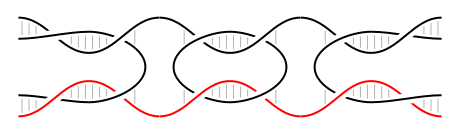
\includegraphics[width=\textwidth]{./figures/dao-dae/dae.pdf}
				\caption{DAE.}
				\label{fig:dao}
			\end{subfigure}
			\begin{subfigure}[b]{0.405\textwidth}
				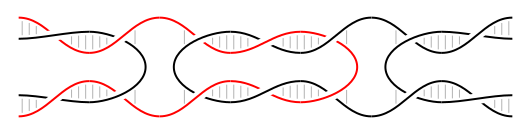
\includegraphics[width=\textwidth]{./figures/dao-dae/dao.pdf}
				\caption{DAO.}
				\label{fig:dae}
			\end{subfigure}
			\caption{DAO vs. DAE.}
			\label{fig:dao-dae}
		\end{center}
		\end{figure}
		
		
		
		DAE molecules seem to be the most promising % citovat tunu praktickejch článků
		thus chapter \ref{chap:problems} will be dedicated spacially to these molecules.
		
		% Biostep complexity $O(1)$ in particular cases.
		
		% DAO vs. DAE units. Winfree pg 36 -- sizes of DAE and a better picture, pg 37 -- comparison of DAO/DAE in a lattice, explanation pg 43.
		
		% Seeman, Fu \cite{seeman93}, is the picture of DAO strange?
		
		% Important notes in 3.2.5 Winfree -- single side hybridization -- how to avoid.

% Hasentiles! Hase = zajíc (D)

\section{Wang-tile models}

\subsection{Definition}
	
	% Winfree pg 56
	
	We will rather define Wang tile models less formally because it will be clear what they mean and excessive formality could cause confusions.
	
	Wang tile is a square tile with one color (also index, glue) from a finite nonempty set $I$ on each its edge\footnote{Tiles keep orientation, they are {\em not} allowed to rotate nor reflect.}, let us denote (nonempty) set of all available tiles $T$. Wang tiling is a mapping ${\cal T}: (\Z^2) \rightarrow T$ with restrictions: neighboring tiles must have the same color on the adjacent edge and its domain is required to be (topologically) connected. Wang tiling ${\cal T}_2$ is called {\em reachable} from Wang tiling ${\cal T}_1$ iff ${\cal T}_1 \subseteq {\cal T}_2$. A tiling $\cal T$ is called {\em terminal} iff there does not exist any sharply bigger tiling reachable from $\cal T$. %!% říct jaký to uspořádání je, že má minimální prvek
	
	Winfree extends this definition for DNA tile assembly purposes and introduces Abstract Tile Assembly Model (aTAM). Additionally
	\begin{itemize}
		\item every color $c$ is associated with a nonnegative integer $g(c)$ which will also be referred to as {\em glue strength},
		\item there exists an empty color denoted by $\epsilon$ which can be neighboring with arbitrary color,
		\item tiling is only allowed to grow
		\begin{itemize}
			\item from a special initial tile denoted by $t_0$ from $(0,0)$ ({\em initial configuration}),
			\item one tile per step,
			\item the sum of just connected glues must be greater or equal to given integer treshold\footnote{Interesting to study are small numbers like $1$, $2$; there are different results in Section \ref{sec:wang_power}}, so called {\em temperature}, denoted by $\tau$.
		\end{itemize}
	\end{itemize}
	Reachability relation will be restricted accordingly to these rules, {\em reachable in (tilesystem) $T$} will mean reachable from initial configuration, same for {\em terminal tiling in (tilesystem) $T$}.
	
	Similarly to Turing machines, tilesystem $T$ will be called:
	\begin{description}
		\item[Deterministic] iff there exists unique terminal tiling in $T$. % (in other words, reachability relation has one minimal/maximal member).
		\item[Non-deterministic] iff it has no other restrictions. % no ...
		\item[Probabilistic] iff every possible step in every stage has defined probability. See Note \ref{note:tilesystems} for a proposal how the probability could be defined.
	\end{description}
	
	\begin{note}\label{note:tilesystems}
		If there is a unique place and a unique tile the probability is clearly $1$. If there is a unique place but there are more candidate tiles, the probability $\prob_C(t)$ of connecting tile $t$ should be distributed to these tiles somehow according to their concentration ratio (denoted by $\prob_0(t)$) and their total connectible glue strength (denoted by $G(t)$). Most straightforward is weighted average:
		\begin{equation*}
			\prob_C(t) = \frac{G(t)\cdot\prob_0(t)}{\sum\limits_{u\textnormal{ possible tile}}G(u)\cdot\prob_0(u)}
		\end{equation*}
		In the most general case there are more places, each having several candidates. The probability $\prob_C(t,i)$ of connecting tile $t$ on place $i$ can be defined as weighted average again, now with one more sum over all possible places:
		\begin{equation*}
			\prob_C(t,i) = \frac{G(t,i)\cdot\prob_0(t)}{\sum\limits_{j\textnormal{ possible place}}\quad\sum\limits_{u\textnormal{ possible tile}\atop\textnormal{on place }j}G(u,j)\cdot\prob_0(u)}
		\end{equation*}
	\end{note}

\subsection{Computational power}\label{sec:wang_power}
	
	The most exciting thing about aTAM is that
	\begin{itemize}
		\item it is known to be capable of universal computation at temperature $2$ in 2D,
		\item also at temperature $1$ in 3D,
		\item but it is not known to be universal or not at temperature $1$ in 2D\footnote{Universality has been reached only with modifications to the original model, see \cite{stage_assembly}, \cite{active_tiles}.}.
	\end{itemize}
	Let us show known results in a table.
	
	\begin{center}
	\begin{tabular}{|| c || c | c | c ||}
		\hline\hline
		~ & \multicolumn{2}{c|}{\bf $n\times n$ squares} & {\bf Computational} \\
		~ & \multicolumn{1}{c}{LB} & \multicolumn{1}{c|}{UB} & {\bf Power}\\
		\hline
		$\tau=2$, 2D & \multicolumn{2}{c|}{See \cite{square_lb}, $\Theta(\frac{\log n}{\log\log n})$, see \cite{square_ub}} & Universal, see \cite{winfree_phd} \\
		\hline
		$\tau=1$, 3D & $\Omega(\frac{\log n}{\log\log n})$, see \cite{square_lb} & $O(\log n)$, see \cite{cook_temp1} & Universal, see \cite{cook_temp1} \\
		\hline
		$\tau=1$, 2D & $\Omega(\frac{\log n}{\log\log n})$, see \cite{square_lb} & $2n-1$, see \cite{square_lb} & Unknown \\
		\hline\hline
	\end{tabular}
	\end{center}

\subsection{Turing universality of 2D tiles at $\tau=2$}
	
	Here we propose an alternative and more straightforward 2D tilesystem denoted by ${\cal T}_{TM}$ which directly simulates Turing machine at $\tau=2$ proving Turing universality of this model, see Figures \ref{fig:tileset1} and \ref{fig:tileset2}. All tiles are described within figures.
	\begin{remark}
		This tilesystem can simulate deterministic Turing machine as well as non-deter\-ministic or probabilistic if we consider probabilistic tilesystem, all in $O(1)$ biosteps.
	\end{remark}
	The worst case occurs when the head is changing its step direction because all the rest of the tape must be copied. Following lemma gives upper bound for binding complexity as well as for the other studied complexities.
	\begin{lemma}
	\label{lem:TM_bound}
		Studied complexities in tilesystem ${\cal T}_{TM}$ are bounded:
		\begin{description}
			\item[Biostep] $Bs(n) \in O(1)$.
			\item[Binding] $Bnd(n) \in O(t^2(n))$ where $t(n)$ denotes time of the simulated Turing machine.
			\item[Tile] $Ti(n) \in O(n)$.
			\item[Glue] $Gl(n) \in O(n)$.
		\end{description}
	\end{lemma}
	\begin{proof}
		~
		\begin{description}
			\item[Biostep] all tiles are designed to operate altogether thus only constant number of biosteps is needed.
			\item[Binding] all Turing machine steps are simulated one-to-one or one-to-constant number of bindings with only one exception which is tape-copying as soon as head changes its direction. The length of %!% popsaný
			used tape is $\leq t(n)$. Every copied length is thus bounded by $t(n) + C$ where $C$ is a constant, copying process is thus bounded by $2(t(n)+C)$ bindings. Copying occurs maximally once per simulated step thus number of copying is bounded by $t(n)$. Altogether number of bindings is bounded by $2(t(n)+C)\cdot t(n) \in O(t^2(n))$.
			\item[Tile] number of non-input tiles is constant, it is proportional to Turing machine size which is constant. There must only be prepared $n$ special input tiles thus $Ti(n) \in O(n)$.
			\item[Glue] from Lemma \ref{lem:ti_gl} follows that $Gl(n) \leq 4Ti(n)$ and I really need $n$ glues to connect input tiles uniquely, $Gl(n)\in O(n)$.
		\end{description}
	\end{proof}
	\begin{cor}
	\label{cor:poly_resist}
		All classes resistant to polynomial slowdown ($\P$, $\ZPP$, $\RP$, $\BPP$, $\NP$, \ldots) remain preserved for all studied complexities.
	\end{cor}
	
	\begin{figure}[h]
	\begin{center}
		\includegraphics{./figures/tiles1.pdf}
		\caption{Tileset 1/2. Symmetric tiles are considered.}
		\label{fig:tileset1}
	\end{center}
	\end{figure}
	
	\begin{figure}[h]
	\begin{center}
		\includegraphics{./figures/tiles2.pdf}
		\caption{Tileset 2/2. Symmetric tiles are considered.}
		\label{fig:tileset2}
	\end{center}
	\end{figure}

\subsection{Feasibility of the class $\BPP$}
	
	Remind that every language from $\BPP$ is dedidable on a PTM in polynomial time which means that probability of correct result is $> \nicefrac{2}{3}$. Note that one can reach probability of correct result higher than arbitrary constant $<1$ by constant number of iterations. Thus it is reasonable to consider $\BPP$ as practically feasible\footnote{Considering even Quantum Turing machine to be practically feasible, $\BQP$ (a superset of $\BPP$) would be practically feasible. Note that due to Shor's algorithm \cite{shor94}, Integer Factorization Problem belongs to $\BQP$ but it is assumed that it does not belong to $\BPP$. Thus $\BPP$ is assumed to be proper subset of $\BQP$.}.
	
	Here we introduce a similar proposal for feasibility of DNA algorithms. In Remark \ref{rem:stud_compl} we proposed that feasible algorithms' biostep complexity must comply $Bs(n)\in O(1)$ which is proved in Lemma \ref{lem:TM_bound} for tilesystem ${\cal T}_{TM}$. There are also practical reasons for limitation of the other complexities, not yet so sharp, so we will require them to be polynomial. Corollary \ref{cor:poly_resist} states preserving of classes $\P$, $\ZPP$, $\RP$, $\BPP$, $\NP$, \ldots in tilesystem ${\cal T}_{TM}$ which justifies Corollary \ref{cor:bpp_feas}.
	
	\begin{thesis}   %!% conjecture nebo lépe?
		Feasible DNA algorithms comply $Bs(n)\in O(1)$; $Bnd(n),\,Ti(n),\,Gl(n)\in \P$.   %!% možná postačí pro poly algoritmus mín jak \P tile a glue !!! ale spíš ne
	\end{thesis}
	
	\begin{cor}
	\label{cor:bpp_feas}
		$\BPP$ is feasible in 2D at temperature $\tau=2$.
	\end{cor}
	
	\begin{note}
		Remind that $\P$, $\ZPP$, $\RP$ and $\coRP \subseteq \BPP$.
	\end{note}
	
	
	
	%~ \begin{thm}   %!% tohle je potřeba někde najít a citovat
		%~ Probabilistic Turing machine can be simulated by probabilistic cellular automaton.
	%~ \end{thm}
	
	%!% popsat co znamená že je něco sestavitelný -- NP, že má něco pst sestavení -- BPP
	
	%!% nák rozumně vysvětlit že \NP se dá na PTM docela dobře spočítat
	% The model can practically handle also $\NP$ languages (not theoretically, of course) because 
	
	%%%%%%%%%%%%%%%%%%%%%%%%%%%%%%%%%%%%%%%%%%%%%%%%%%%%%%%%%%%%%%%%%%%%%%
	
	% error-tolerant rules -- Gacs and Reif, 1988\\



%%% KAPITOLA 2
\chapter{Strand models}

% úvod o kapitole, přehled

Quick overview of considered structures. Winfree's overview (pg 29 -- considered molecules, pg 36 -- sizes of DAE and a better picture, pg 37 -- comparison of DAO/DAE in a lattice, explanation pg 43).

Seeman, Fu and their DAO/DAE in \cite{seeman93}, is the picture of DAO strange?

\section{Adleman's experiment}
	
	Adleman showed in his ground-breaking work, \cite{adleman94}, that DNA molecules are really capable of computation. He exploited that huge parallelism possible in DNA computation for one of the most fundamental NP-complete problems -- the Hamiltonian Path Problem (HPP) in directed graph with designated vertices $v_{begin}$ and $v_{end}$.
	
	Let us remind this type of HPP. Given a directed graph $G_n$ with $n$ vertices and two designated vertices $v_{begin}$ and $v_{end}$, the problem is to answer whether there exists an oriented path from $v_{begin}$ to $v_{end}$ through the graph such that the path visits every vertex. Note that {\em path} cannot visit any vertex more than once from definition.
	
	\begin{figure}[H]
	\begin{center}
		\includegraphics{./figures/adleman_graph.pdf}
		\caption{Adleman's original graph.}
		\label{fig:adleman_graph}
	\end{center}
	\end{figure}
	
	Adleman originally used a graph with seven vertices shown in figure \ref{fig:adleman_graph}. It can be seen that the path $0 \rightarrow 1 \rightarrow 2 \rightarrow 3 \rightarrow 4 \rightarrow 5 \rightarrow 6$ is Hamiltonian\footnote{Note that it can be re-labelled such a nice way without loss of generality.}.
	
	Adleman first presents this non-deterministic five-step algorithm, whose steps are then described in terms of DNA manipulations:
	\begin{description}
		\item[Step 1] Generate random paths through the graph.
		\item[Step 2] Keep only those paths that begin with $v_{begin}$ and end with $v_{end}$.
		\item[Step 3] If the graph has $n$ vertices, then keep only those paths that enter exactly $n$ vertices.
		\item[Step 4] Keep only those paths that enter all of the vertices of the graph at least once.
		\item[Step 5] If any paths remain, say ``Yes''; otherwise, say ``No.''\footnote{This is the original version, I would rectify the fifth step: If any paths remain, say ``Yes''; otherwise, say ``{\em I do not know.}'' That is because NP problem gives answer ``Yes'' iff there {\em exists} supporting solution. To say ``No'' one needs to show that {\em all} solutions do not satisfy. That is exactly the difference between NP and co-NP.}
	\end{description}
	To see % sloveso od insight ?
	how DNA can compute, let us describe this example more precisely. The computation itself (I mean the inception of the final solution) is hidden in Step 1. Each vertex $i$ is associated with a random\footnote{We will expect those sequences to be different enough.} $20$-mer sequence of DNA, let us denote its $5'\rightarrow 3'$ orientation by $O_i$, its 10-mer prefix by $p_i$ and its 10-mer suffix by $q_i$. Each edge $i\rightarrow j$ is then associated with $\overline{q_i p_j}$ sequence with reverse backbone orientation ($3'\rightarrow 5'$) where $\overline{q_i}$ stands for Watson-Crick complementary word. There is an exception for $i=begin$ and $j=end$: instead of $\overline{q_{begin} p_j}$ there is $\overline{O_{begin} p_j}$ and in a similar way for $j=end$.
	
	\begin{figure}[H]
	\begin{center}
		\includegraphics{./figures/adleman_strands.pdf}
		\caption{Example of assigned sequences.}
		\label{fig:adleman_strands}
	\end{center}
	\end{figure}
	
	It can be easily seen that all correctly bonded double-strands correspond with a valid path in $G_n$. Moreover, all complete double-strands represent a valid path from $v_{begin}$ to $v_{end}$ through $G_n$.
	
	All the other steps are fully described in \cite{adleman94}. The most important thing is that the most time-demanding step is Step 4. In this step one has to purify the product of Step 3 with a biotin-avidin magnetic beads system. This process extracts consequently for every vertex $i$ only those DNA strands which contain a substring representing vertex $i$. Thus its biostep complexity is $O(n)$. If we assume that one biostep takes at least tens of minutes and it should be performed repeatedly to avoid errors, we can conclude that $O(n)$ is just too much\footnote{Winfree, \cite{winfree_phd}, gives a positive solution.}.

\section{Single-stranded molecules}
	
	SAT in $O(1)$ biosteps etc.

\section{Double-stranded molecules}
	
	\subsection{Linear strands}
		
		Equivalent to regular languages.
	
	\subsection{Dendrimer structures}
		
		Equivalent to context-free languages.

\section{Double crossover molecules}
	
	Equivalent to recursively enumerable languages (Turing universal). Important notes in 3.2.5 Winfree -- single side hybridization -- how to avoid. Tricky solution of Hamiltonian Path Problem.

%%% KAPITOLA 3
\chapter{Wang tile models}   % Hasentiles! Hase = zajíc (D)

\section{Definition}
	
	More abstract model where one handles only with ``glues'' on edges of Wang tiles. Define {\em temperature}.

\section{Computational power}
	
	Give table of Turing universality \cite{cook_temp1}.
	
	See \cite{winfree_phd}. Many other results in \cite{cook_temp1}, \cite{stage_assembly}, \cite{square_lb}, \cite{square_ub} \ldots
	
	\subsection{Turing universality of 2D tiles at $T=2$}
		
		\begin{figure}[H]
		\begin{center}
			\includegraphics{./figures/tiles1.pdf}
			\caption{Tileset 1/2.}
		\end{center}
		\end{figure}
		
		\begin{figure}[H]
		\begin{center}
			\includegraphics{./figures/tiles2.pdf}
			\caption{Tileset 2/2.}
		\end{center}
		\end{figure}
	
	%%%%%%%%%%%%%%%%%%%%%%%%%%%%%%%%%%%%%%%%%%%%%%%%%%%%%%%%%%%%%%%%%%%%%%
	
	error-tolerant rules -- Gacs and Reif, 1988\\


%%% KAPITOLA 4
\chapter{Results}

\section{Abstract model for DAE units}

% \section{Abstract model for DAE units}

It is better to draw easier-to-understand pictures. Explanation: \ldots Call those DNA sequences ``glues''.

In following examples this model will be set up to act similarly like NP: $\exists y \; R(x,y)$. Although existence is not sure, it is very likely. Predicate $R$ will be ``enumerable in polynomial time'' for $x \in L$. In this context, {\em enumerable in polynomial time} will mean number of bindings, not number of biosteps. This can be assumed due to Turing universality of this model in $O(1)$ biosteps -- biostep complexity is not restrictive\footnote{From Turing's thesis, Turing machine is the most universal model.} and will be required to be $O(1)$ due to its lab complexity. On the other hand the binding complexity will be very important, we will be interested even in constants. This is because the less binding complexity, the less probability of error.

% diskutovat pravděpodobnost objevení vs. neobjevení $y$ !!! dát odkaz do footnote
% odhady se dají zmenšit pomocí #E místo #V^2

Define (slightly more correctly) binding complexity of this model as the number of bindings. Only the biggest term will be considered but even with constant.

\begin{figure}[h]
\begin{center}
	\begin{subfigure}[b]{0.31\textwidth}
		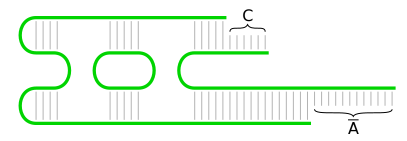
\includegraphics[width=\textwidth]{./figures/tile_model/DNA_struct.pdf} % 115mm
		\caption{Corner DAE unit}
		\label{fig:DNA_struct}
	\end{subfigure}%
	%add desired spacing between images, e. g. ~, \quad, \qquad etc.
	%(or a blank line to force the subfigure onto a new line)
	\begin{subfigure}[b]{0.472\textwidth}
		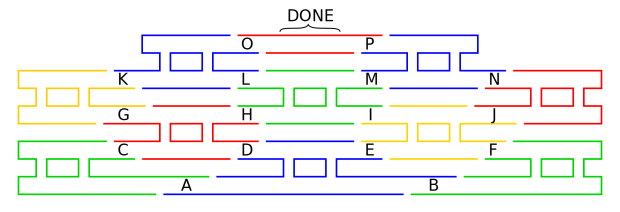
\includegraphics[width=\textwidth]{./figures/tile_model/DNA_assembly.pdf} % 175mm
		\caption{Whole self-assembly}
		\label{fig:DNA_assembly}
	\end{subfigure}
	\begin{subfigure}[b]{0.190\textwidth}
		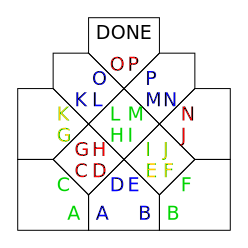
\includegraphics[width=\textwidth]{./figures/tile_model/abstract_model.pdf} % 70mm
		\caption{Abstract model}
		\label{fig:abstract_model}
	\end{subfigure}
	\caption{Evolution of abstract model from DAE units to tiles.}
	\label{fig:evolution}
\end{center}
\end{figure}



\section{Graph 3-coloring}

\input{./include/4-results_2-3-color.tex}


\newpage
\section{Graph isomorphism}

\input{./include/4-results_3-isomorph.tex}


\newpage
\section{$k$-clique}

\input{./include/4-results_4-k-clique.tex}


%%% ZÁVĚREM
\cleardoublepage\phantomsection   % cleardoublepage a phantomsection udělají že odkaz z obsahu vede NAD nadpis, jinak vede POD
\addcontentsline{toc}{chapter}{Epilog}
\chapter*{Epilog}
	
	The very last section to be done.

%%% LITERATURA
% \renewcommand\bibname{Literatura}
\input{./include/n-biblio.tex}


%%%%%%%%%%%%%%%%%%%%%%%%%%%%%%%%%%%%%%%%%%%%%%%%%%%%%%%%%%%%%%%%%%%%%%%%
%     K O N E C   P R Á C E                                            %
%%%%%%%%%%%%%%%%%%%%%%%%%%%%%%%%%%%%%%%%%%%%%%%%%%%%%%%%%%%%%%%%%%%%%%%%


\end{document}